%%%%%%%%%%%%%%%%%%%%%%%%%%%%%%%%%%%%%%%%%
% Beamer Presentation
% LaTeX Template
% Version 1.0 (10/11/12)
%
% This template has been downloaded from:
% http://www.LaTeXTemplates.com
%
% License:
% CC BY-NC-SA 3.0 (http://creativecommons.org/licenses/by-nc-sa/3.0/)
%
%%%%%%%%%%%%%%%%%%%%%%%%%%%%%%%%%%%%%%%%%

%----------------------------------------------------------------------------------------
%	PACKAGES AND THEMES
%----------------------------------------------------------------------------------------

\documentclass{beamer}

\mode<presentation> {

% The Beamer class comes with a number of default slide themes
% which change the colors and layouts of slides. Below this is a list
% of all the themes, uncomment each in turn to see what they look like.

%\usetheme{default}
%\usetheme{AnnArbor}
%\usetheme{Antibes}
%\usetheme{Bergen}
%\usetheme{Berkeley}
%\usetheme{Berlin}
%\usetheme{Boadilla}
%\usetheme{CambridgeUS}
%\usetheme{Copenhagen}
%\usetheme{Darmstadt}
%\usetheme{Dresden}
%\usetheme{Frankfurt}
%\usetheme{Goettingen}
%\usetheme{Hannover}
%\usetheme{Ilmenau}
%\usetheme{JuanLesPins}
%\usetheme{Luebeck}
\usetheme{Madrid}
%\usetheme{Malmoe}
%\usetheme{Marburg}
%\usetheme{Montpellier}
%\usetheme{PaloAlto}
%\usetheme{Pittsburgh}
%\usetheme{Rochester}
%\usetheme{Singapore}
%\usetheme{Szeged}
%\usetheme{Warsaw}

% As well as themes, the Beamer class has a number of color themes
% for any slide theme. Uncomment each of these in turn to see how it
% changes the colors of your current slide theme.

%\usecolortheme{albatross}
%\usecolortheme{beaver}
%\usecolortheme{beetle}
%\usecolortheme{crane}
%\usecolortheme{dolphin}
%\usecolortheme{dove}
%\usecolortheme{fly}
%\usecolortheme{lily}
%\usecolortheme{orchid}
%\usecolortheme{rose}
%\usecolortheme{seagull}
%\usecolortheme{seahorse}
%\usecolortheme{whale}
%\usecolortheme{wolverine}

%\setbeamertemplate{footline} % To remove the footer line in all slides uncomment this line
%\setbeamertemplate{footline}[page number] % To replace the footer line in all slides with a simple slide count uncomment this line

%\setbeamertemplate{navigation symbols}{} % To remove the navigation symbols from the bottom of all slides uncomment this line
}

\usepackage{plantuml}
\usepackage{biblatex}
\usepackage{graphicx} % Allows including images
\usepackage{booktabs} % Allows the use of \toprule, \midrule and \bottomrule in tables
\usepackage{bookmark}
\usepackage{biblatex}
\addbibresource{../bib/ijcai11.bib}

\newif\iflspCommEx% <lspCommEx>
\newif\ifvsceArch% <vsceArch>
\newif\ifdaGdb% <daGdb>
\newif\ifmnProb% <mnProb>
\newif\ifsolMnProb% </solMnProb>
\newif\ifsolDbg% </solDbg>
\newif\ifiro% </iro>
\newif\ifauto% </auto>
\newif\ifmyc% </myc>
\newif\ifmycext% </mycext>
\newcommand{\loadFig}[1]{{% \inputbetweentag{<tag>}{<filename>}
  \expandafter\let\csname if#1\endcsname\iftrue% Make "tag" true
  %Figure file
% dont use _ or whitespace in tags
% every tag added here be sure to add into figtag.tex

\iflspCommEx% <lspCommEx>
\begin{figure}
    \begin{plantuml}
      @startuml
      skinparam defaultTextAlignment center
      skinparam SequenceMessageAlign center
      actor User
      participant DevTool
      participant LangServer
      activate User
      activate DevTool
      activate LangServer
      User -> DevTool: open document
      DevTool -> LangServer: Notification: textDocument/didOpen; Params: document
      User -> DevTool: edit document
      DevTool -> LangServer: Notification: textDocument/didChange; Params: {documentURI, changes}
      LangServer -> DevTool: Notification: textDocument/publishDiagnostics; Params: Diagnostic[]
      User -> DevTool: execute goto definition
      DevTool -> LangServer: Request: textDocument/definition; Params: {documentURI, position}
      LangServer -> DevTool: Response: textDocument/definition; Result: Location
      User -> DevTool: close document
      DevTool -> LangServer: Notification: textDocument/didClose; Params: documentURI
      deactivate LangServer
      deactivate DevTool
      deactivate User
      @enduml
    \end{plantuml}
    \caption{Example of communication between the LSP client and server \cite{lsp}}
    \label{lspCommEx}
\end{figure}
\fi% </lspCommEx>

\ifvsceArch% <vsceArch>
\begin{figure}
    \begin{plantuml}
      @startuml
      skinparam defaultTextAlignment center
      skinparam SequenceMessageAlign center
      skinparam linetype ortho
      left to right direction
        rectangle "VS Code" {
        rectangle "Extension Host" {
        rectangle hlc [
        HTML Language Client
        ]
        rectangle plc [
        PHP Language Client
        ]
        }
        }
        
        rectangle hls [
        HTML Language Server
        ]
        rectangle pls [
        PHP Language Server
        ]
        
        hlc --> hls
        hls --> hlc: LSP over JSON-RPC
        plc --> pls
        pls --> plc: LSP over JSON-RPC
      @enduml
    \end{plantuml}
    \caption{Integration of extension into VSCode\cite{vsclspextman}}
    \label{vsceArch}
\end{figure}
\fi% </vsceArch>

\ifdaGdb% <daGdb>
\begin{figure}
    \begin{plantuml}
    @startuml
      skinparam defaultTextAlignment center
      skinparam SequenceMessageAlign center
      actor User
      participant DevTool
      participant DebugAdapter
      participant Debugger
      User -> DevTool : start debugging
      activate DevTool
      DevTool -> DebugAdapter: start debug adapter
      activate DebugAdapter
      DevTool -> DebugAdapter: initialize request
      DebugAdapter -> Debugger: start gdb
      activate Debugger
      DebugAdapter -> DevTool: response: capabilities
      DebugAdapter --> DevTool: initalized event
      User -> DevTool : set breakpoint
      DevTool -> DebugAdapter: setBreakpoints request
      DebugAdapter -> Debugger: break "hello.c:main:4"
      DebugAdapter -> DevTool: response: breakpoints
      User -> DevTool : run
      DevTool -> DebugAdapter: launch request
      DebugAdapter -> Debugger: file "a.out"
      DebugAdapter -> Debugger: run
      DebugAdapter -> DevTool: response: status
      deactivate DevTool
      deactivate DebugAdapter
      deactivate Debugger
    @enduml
    \end{plantuml}
    \caption{Example of communication between IDE's generic debugger and GDB via Debug adapter \cite{dap}}
    \label{daGdb}
\end{figure}
\fi% </daGdb>

\ifmnProb% </mnProb>
\begin{figure}
    \begin{plantuml}
      @startuml
      skinparam defaultTextAlignment center
      skinparam linetype polyline
      left to right direction
      rectangle Languages {
        usecase "JS" as js
        usecase "Python" as py
        usecase "Java" as jav
      }
      rectangle IDEs {
        usecase "VSCode" as vsc
        usecase "Eclipse" as ec
        usecase "Vim" as vim
      }
      js --> vsc
      js --> ec
      js --> vim
      py --> vsc
      py --> ec
      py --> vim
      jav --> vsc
      jav --> ec
      jav --> vim
      @enduml
    \end{plantuml}
    \caption{The {\it m+n} problem\cite{vsclspextman}}
    \label{mnProb}
\end{figure}
\fi% </mnProb>

\ifsolMnProb% </solMnProb>
\begin{figure}
    \begin{plantuml}
      @startuml
      skinparam defaultTextAlignment center
      left to right direction
      rectangle LSP_Server {
        usecase "JS" as js
        usecase "Python" as py
        usecase "Java" as jav
      }
      rectangle LSP
      rectangle LSP_Client {
        usecase "VSCode" as vsc
        usecase "Eclipse" as ec
        usecase "Vim" as vim
      }
      js --> LSP
      py --> LSP
      jav --> LSP
      LSP --> vsc
      LSP --> ec
      LSP --> vim
      @enduml
    \end{plantuml}
    \caption{Solution to {\it m+n} problem\cite{vsclspextman}}
    \label{solMnProb}
\end{figure}
\fi% </solMnProb>

\ifsolDbg% </solDbg>
\begin{figure}
    \begin{plantuml}
      @startuml
      skinparam defaultTextAlignment center
      left to right direction
      rectangle "IDE (with Generic Debugger)" {
        usecase "VSCode" as vsc
        usecase "Eclipse" as ec
        usecase "Vim" as vim
      }
      rectangle DA
      rectangle JS_DA
      rectangle Python_DA
      rectangle Java_DA
      rectangle JS_Debugger
      rectangle Python_Debugger
      rectangle Java_Debugger
      vsc --> DA
      ec --> DA
      vim --> DA
      DA --> JS_DA
      DA --> Python_DA
      DA --> Java_DA
      JS_DA --> JS_Debugger 
      Python_DA --> Python_Debugger
      Java_DA --> Java_Debugger
      @enduml
    \end{plantuml}
    \caption{Solution for debugging support\cite{dap}}
    \label{solDbg}
\end{figure}
\fi% </solDbg>

\ifiro% </iro>
\begin{figure}
    \begin{plantuml}
      @startuml
      skinparam defaultTextAlignment center
      left to right direction
      rectangle IRO
      rectangle "Format" {
        usecase "Texmate" as tm
        usecase "Atom" as at
        usecase "Ace" as ace
        usecase "Sublime3" as sub3
      }
      rectangle "Users" {
        usecase "VSCode" as vsc
        usecase "Eclipse" as ec
        usecase "Github" as gh
        usecase "Atom editor" as atsh
        usecase "Ace editor" as acesh
        usecase "Sublime editor" as sub3sh
      }
      IRO --> tm
      IRO --> at
      IRO --> ace
      IRO --> sub3
      tm --> vsc
      tm --> ec
      tm --> gh
      at --> gh
      at --> atsh
      ace --> acesh
      sub3 --> sub3sh
      @enduml
    \end{plantuml}
    \caption{{\it IRO}\cite{iro} and supported grammar formats}
    \label{iro}
\end{figure}
\fi% </iro>

\ifauto% </auto>
\begin{figure}
    \begin{plantuml}
      @startuml
      skinparam defaultTextAlignment center
      package "Template project" as TPrj {
        [LSP Client with entry points]
        [LSP Server with entry points]
      }
      file "Entry point list YAML file" as EPY
      file "Language Configuration YAML file" as LCY
      rectangle "Automation script" {
      database "Automation script module" as AutoMod
      package "LSP project" as LSPrj {
        [LSP Client]
        [LSP Server]
      }
      database "npm installer" as npi
      package "Precompiled LSP project" as LSPPrj {
        [LSP Client]
        [LSP Server]
        [npm modules]
      }
      database "VSCE" as vsce
      }
      folder "LSP Extension" as LSPex  
      TPrj --> AutoMod
      EPY --> AutoMod
      LCY --> AutoMod
      AutoMod --> LSPrj
      LSPrj --> npi
      npi --> LSPPrj
      LSPPrj --> vsce
      vsce --> LSPex
      @enduml
    \end{plantuml}
    \caption{Automation of generation of LSP extension}
    \label{auto}
  \end{figure}
\fi% </auto>

\ifmyc% </myc>
\begin{figure}
    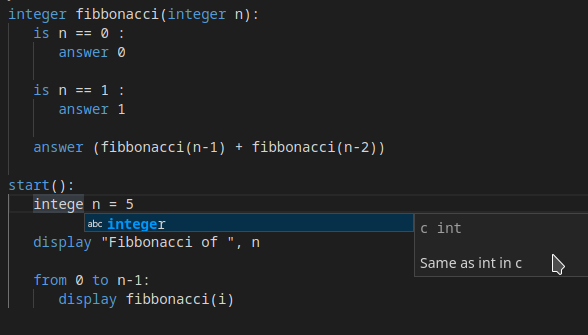
\includegraphics[width=\linewidth]{../fig/myc.png}
    \caption{Keyword syntax Highlighting, auto completion and inline documentation}
    \label{myc}
\end{figure}
\fi% </myc>

\ifmycext% </mycext>
\begin{figure}
    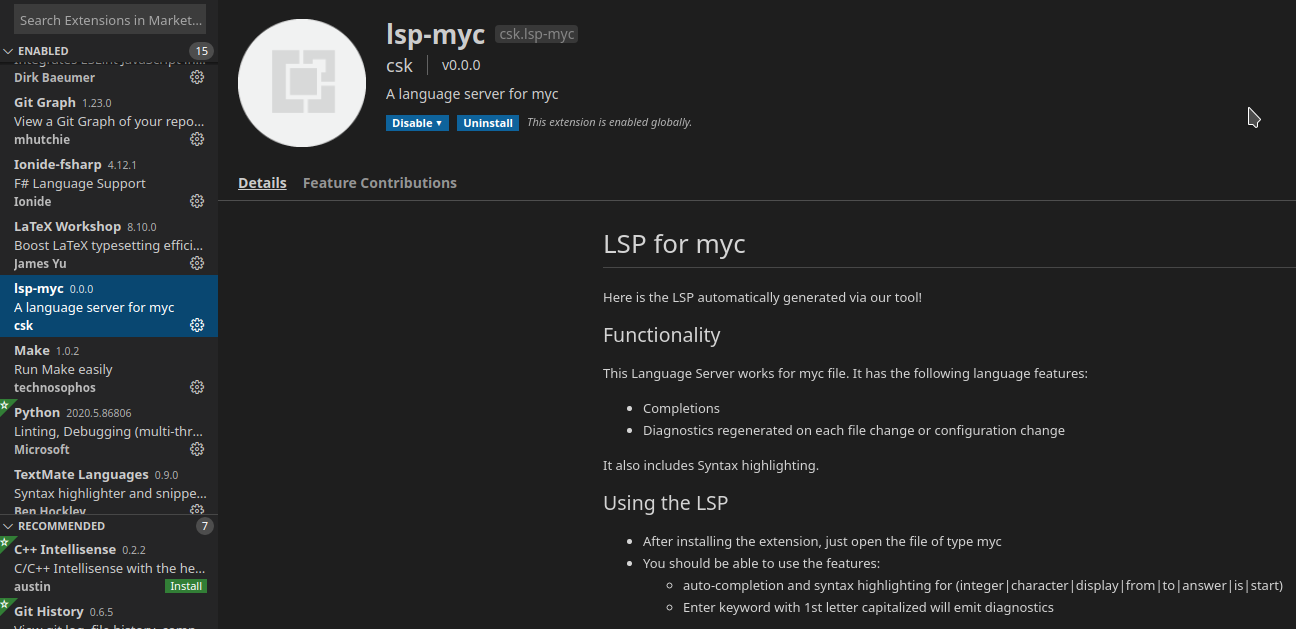
\includegraphics[width=\linewidth]{../fig/mycext.png}
    \caption{Extension for LSP of {\it myc} installed in VSCode}
    \label{mycext}
\end{figure}
\fi% </mycext>}
}% Input file
%----------------------------------------------------------------------------------------
%	TITLE PAGE
%----------------------------------------------------------------------------------------

\title[Short title]{Full Title of the Talk} % The short title appears at the bottom of every slide, the full title is only on the title page

\author{John Smith} % Your name
\institute[UCLA] % Your institution as it will appear on the bottom of every slide, may be shorthand to save space
{
University of California \\ % Your institution for the title page
\medskip
\textit{john@smith.com} % Your email address
}
\date{\today} % Date, can be changed to a custom date

\begin{document}

\begin{frame}
\titlepage % Print the title page as the first slide
\end{frame}

\begin{frame}
\frametitle{Overview} % Table of contents slide, comment this block out to remove it
\tableofcontents % Throughout your presentation, if you choose to use \section{} and \subsection{} commands, these will automatically be printed on this slide as an overview of your presentation
\end{frame}

%----------------------------------------------------------------------------------------
%	PRESENTATION SLIDES
%----------------------------------------------------------------------------------------

%------------------------------------------------
\section{First Section} % Sections can be created in order to organize your presentation into discrete blocks, all sections and subsections are automatically printed in the table of contents as an overview of the talk
%------------------------------------------------

\subsection{Subsection Example} % A subsection can be created just before a set of slides with a common theme to further break down your presentation into chunks

\begin{frame}
\frametitle{Paragraphs of Text}
Sed iaculis dapibus gravida. Morbi sed tortor erat, nec interdum arcu. Sed id lorem lectus. Quisque viverra augue id sem ornare non aliquam nibh tristique. Aenean in ligula nisl. Nulla sed tellus ipsum. Donec vestibulum ligula non lorem vulputate fermentum accumsan neque mollis.\\~\\

Sed diam enim, sagittis nec condimentum sit amet, ullamcorper sit amet libero. Aliquam vel dui orci, a porta odio. Nullam id suscipit ipsum. Aenean lobortis commodo sem, ut commodo leo gravida vitae. Pellentesque vehicula ante iaculis arcu pretium rutrum eget sit amet purus. Integer ornare nulla quis neque ultrices lobortis. Vestibulum ultrices tincidunt libero, quis commodo erat ullamcorper id.
\end{frame}

%------------------------------------------------

\begin{frame}
\frametitle{Bullet Points}
\begin{itemize}
\item Lorem ipsum dolor sit amet, consectetur adipiscing elit
\item Aliquam blandit faucibus nisi, sit amet dapibus enim tempus eu
\item Nulla commodo, erat quis gravida posuere, elit lacus lobortis est, quis porttitor odio mauris at libero
\item Nam cursus est eget velit posuere pellentesque
\item Vestibulum faucibus velit a augue condimentum quis convallis nulla gravida
\end{itemize}
\end{frame}

%------------------------------------------------

\begin{frame}
\frametitle{Blocks of Highlighted Text}
\begin{block}{Block 1}
Lorem ipsum dolor sit amet, consectetur adipiscing elit. Integer lectus nisl, ultricies in feugiat rutrum, porttitor sit amet augue. Aliquam ut tortor mauris. Sed volutpat ante purus, quis accumsan dolor.
\end{block}

\begin{block}{Block 2}
Pellentesque sed tellus purus. Class aptent taciti sociosqu ad litora torquent per conubia nostra, per inceptos himenaeos. Vestibulum quis magna at risus dictum tempor eu vitae velit.
\end{block}

\begin{block}{Block 3}
Suspendisse tincidunt sagittis gravida. Curabitur condimentum, enim sed venenatis rutrum, ipsum neque consectetur orci, sed blandit justo nisi ac lacus.
\end{block}
\end{frame}

%------------------------------------------------

\begin{frame}
\frametitle{Multiple Columns}
\begin{columns}[c] % The "c" option specifies centered vertical alignment while the "t" option is used for top vertical alignment

\column{.45\textwidth} % Left column and width
\textbf{Heading}
\begin{enumerate}
\item Statement
\item Explanation
\item Example
\end{enumerate}

\column{.5\textwidth} % Right column and width
Lorem ipsum dolor sit amet, consectetur adipiscing elit. Integer lectus nisl, ultricies in feugiat rutrum, porttitor sit amet augue. Aliquam ut tortor mauris. Sed volutpat ante purus, quis accumsan dolor.

\end{columns}
\end{frame}

%------------------------------------------------
\section{Second Section}
%------------------------------------------------

\begin{frame}
\frametitle{Table}
\begin{table}
\begin{tabular}{l l l}
\toprule
\textbf{Treatments} & \textbf{Response 1} & \textbf{Response 2}\\
\midrule
Treatment 1 & 0.0003262 & 0.562 \\
Treatment 2 & 0.0015681 & 0.910 \\
Treatment 3 & 0.0009271 & 0.296 \\
\bottomrule
\end{tabular}
\caption{Table caption}
\end{table}
\end{frame}

%------------------------------------------------

\begin{frame}
\frametitle{Theorem}
\begin{theorem}[Mass--energy equivalence]
$E = mc^2$
\end{theorem}
\end{frame}

%------------------------------------------------

\begin{frame}[fragile] % Need to use the fragile option when verbatim is used in the slide
\frametitle{Verbatim}
\begin{example}[Theorem Slide Code]
\begin{verbatim}
\begin{frame}
\frametitle{Theorem}
\begin{theorem}[Mass--energy equivalence]
$E = mc^2$
\end{theorem}
\end{frame}\end{verbatim}
\end{example}
\end{frame}

%------------------------------------------------

\begin{frame}
\frametitle{Figure}
Uncomment the code on this slide to include your own image from the same directory as the template .TeX file.
%\begin{figure}
%\includegraphics[width=0.8\linewidth]{test}
%\end{figure}
\end{frame}

%------------------------------------------------

\begin{frame}[fragile] % Need to use the fragile option when verbatim is used in the slide
\frametitle{Citation}
An example of the \verb|\cite| command to cite within the presentation:\\~

This statement requires citation \cite{p1}.
\end{frame}

%------------------------------------------------

\begin{frame}
\frametitle{References}
\footnotesize{
\begin{thebibliography}{99} % Beamer does not support BibTeX so references must be inserted manually as below
\bibitem[Smith, 2012]{p1} John Smith (2012)
\newblock Title of the publication
\newblock \emph{Journal Name} 12(3), 45 -- 678.
\end{thebibliography}
}
\end{frame}

%------------------------------------------------

\begin{frame}
\Huge{\centerline{The End}}
\end{frame}

%----------------------------------------------------------------------------------------

\end{document} 